\section{Auswertung}
\label{sec:Auswertung}

\begin{table}[!htp]
\centering
\caption{Die gemessenen Temperaturen zu den jeweiligen Zeitpunkten.}
\label{tab:zeit-temp}
\begin{tabular}{
  S[table-format=4.0] @{${}\pm{}$} S[table-format=1.0]
  S[table-format=3.1] @{${}\pm{}$} S[table-format=1.1]
  S[table-format=3.1] @{${}\pm{}$} S[table-format=1.1]}
\toprule
\multicolumn{2}{c}{$t$ / s} & \multicolumn{2}{c}{$T_1$ / K} & \multicolumn{2}{c}
{$T_2$ / K} \\
\midrule
  60 & 5 & 297.7 & 0.1 & 295.5 & 0.1 \\
 120 & 5 & 298.4 & 0.1 & 295.0 & 0.1 \\
 180 & 5 & 299.6 & 0.1 & 294.0 & 0.1 \\
 240 & 5 & 301.3 & 0.1 & 292.3 & 0.1 \\
 300 & 5 & 303.0 & 0.1 & 290.5 & 0.1 \\
 360 & 5 & 305.0 & 0.1 & 288.8 & 0.1 \\
 420 & 5 & 306.7 & 0.1 & 287.2 & 0.1 \\
 480 & 5 & 308.5 & 0.1 & 285.5 & 0.1 \\
 540 & 5 & 310.3 & 0.1 & 283.7 & 0.1 \\
 600 & 5 & 311.9 & 0.1 & 282.3 & 0.1 \\
 660 & 5 & 313.4 & 0.1 & 280.8 & 0.1 \\
 720 & 5 & 315.0 & 0.1 & 279.3 & 0.1 \\
 780 & 5 & 316.5 & 0.1 & 277.9 & 0.1 \\
 840 & 5 & 318.1 & 0.1 & 276.4 & 0.1 \\
 900 & 5 & 319.6 & 0.1 & 275.3 & 0.1 \\
 960 & 5 & 321.0 & 0.1 & 274.6 & 0.1 \\
1020 & 5 & 322.3 & 0.1 & 274.0 & 0.1 \\
1080 & 5 & 323.6 & 0.1 & 273.5 & 0.1 \\
\bottomrule
\end{tabular}
\end{table}

\begin{figure}
  \centering
  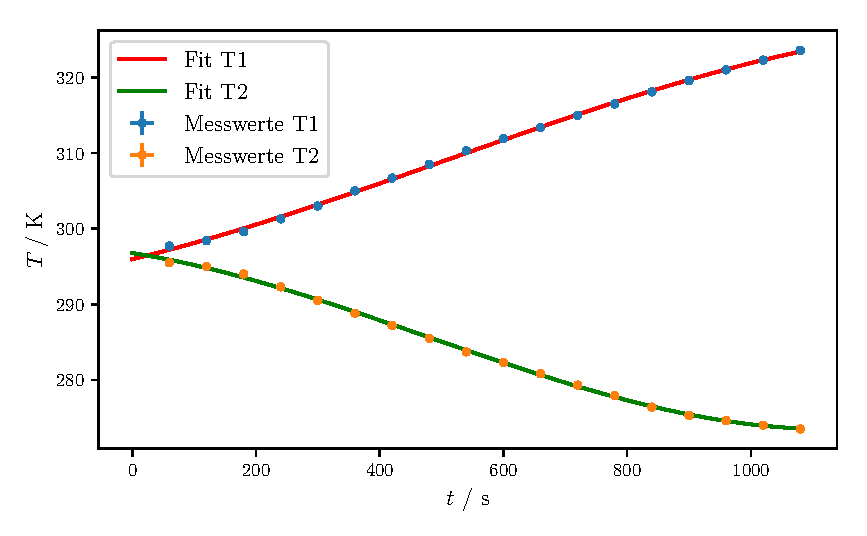
\includegraphics{plot-t-T.pdf}
  \caption{Plot und Fit der Temperaturen in Zeitabhöngigkeit.}
  \label{fig:plot_zeit-temp}
\end{figure}

\begin{figure}
  \centering
  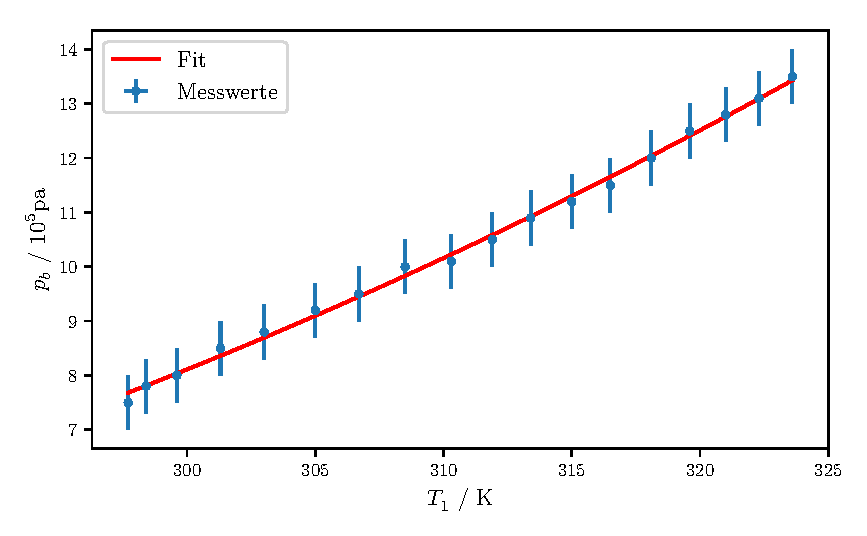
\includegraphics{plot-T-p1.pdf}
  \caption{Die Temperaturen und der Druck in Reservoir 1 gegeneinander aufgetragen.}
  \label{fig:plot_zeit-temp}
\end{figure}

\begin{figure}
  \centering
  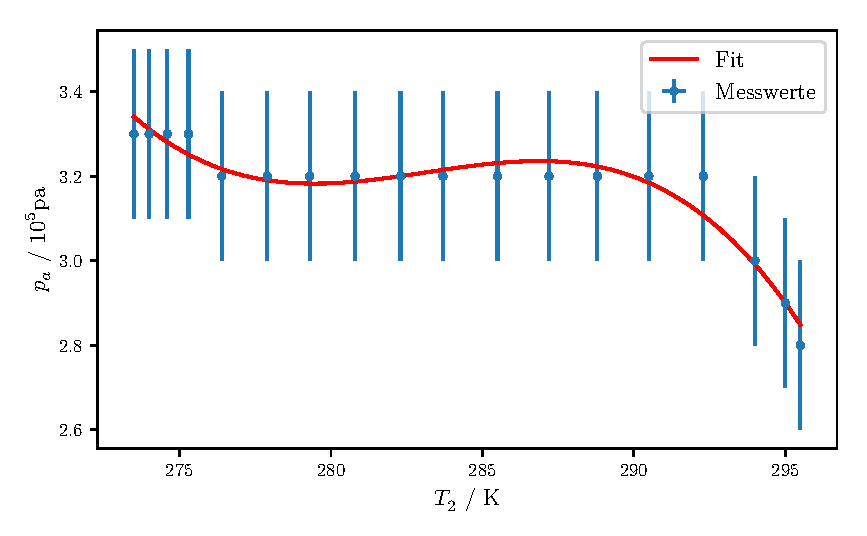
\includegraphics{plot-T-p2.pdf}
  \caption{Die Temperaturen und der Druck in Reservoir 2 gegeneinander aufgetragen.}
  \label{fig:plot_zeit-temp}
\end{figure}

\begin{table}[!htp]
    \centering
    \caption{Temperatur und Druck im Verhältnis.}
    \label{tab:temp-druck}
    \begin{subtable}{0.48\textwidth}
        \begin{tabular}{
            S[table-format=3.1] @{${}\pm{}$} S[table-format=2.1]
            S[table-format=1.1] @{${}\pm{}$} S[table-format=1.1]}
            \toprule
            \multicolumn{2}{c}{$T_1$ / K} & \multicolumn{2}{c}{$p_a$ / $10^5$pa} \\
            \midrule
            297.7 & 0.1 &  7.5 & 0.5 \\
            298.4 & 0.1 &  7.8 & 0.5 \\
            299.6 & 0.1 &  8.0 & 0.5 \\
            301.3 & 0.1 &  8.5 & 0.5 \\
            303.0 & 0.1 &  8.8 & 0.5 \\
            305.0 & 0.1 &  9.2 & 0.5 \\
            306.7 & 0.1 &  9.5 & 0.5 \\
            308.5 & 0.1 & 10.0 & 0.5 \\
            310.3 & 0.1 & 10.1 & 0.5 \\
            311.9 & 0.1 & 10.5 & 0.5 \\
            313.4 & 0.1 & 10.9 & 0.5 \\
            315.0 & 0.1 & 11.2 & 0.5 \\
            316.5 & 0.1 & 11.5 & 0.5 \\
            318.1 & 0.1 & 12.0 & 0.5 \\
            319.6 & 0.1 & 12.5 & 0.5 \\
            321.0 & 0.1 & 12.8 & 0.5 \\
            322.3 & 0.1 & 13.1 & 0.5 \\
            323.6 & 0.1 & 13.5 & 0.5 \\
            \bottomrule
        \end{tabular}
        \caption{Reservoir 1}
    \end{subtable}
    \begin{subtable}{0.48\textwidth}
        \centering
        \begin{tabular}{S[table-format=3.1] c S[table-format=1.1] S[table-format=1.1] c S[table-format=1.1]}
            \toprule
            \multicolumn{2}{c}{$T_2$ / K} & \multicolumn{2}{c}{$p_b$ / $10^5$pa} \\
            \midrule
            295.5 & 0.1 & 2.8 & 0.2 \\
            295.0 & 0.1 & 2.9 & 0.2 \\
            294.0 & 0.1 & 3.0 & 0.2 \\
            292.3 & 0.1 & 3.2 & 0.2 \\
            290.5 & 0.1 & 3.2 & 0.2 \\
            288.8 & 0.1 & 3.2 & 0.2 \\
            287.2 & 0.1 & 3.2 & 0.2 \\
            285.5 & 0.1 & 3.2 & 0.2 \\
            283.7 & 0.1 & 3.2 & 0.2 \\
            282.3 & 0.1 & 3.2 & 0.2 \\
            280.8 & 0.1 & 3.2 & 0.2 \\
            279.3 & 0.1 & 3.2 & 0.2 \\
            277.9 & 0.1 & 3.2 & 0.2 \\
            276.4 & 0.1 & 3.2 & 0.2 \\
            275.3 & 0.1 & 3.3 & 0.2 \\
            274.6 & 0.1 & 3.3 & 0.2 \\
            274.0 & 0.1 & 3.3 & 0.2 \\
            273.5 & 0.1 & 3.3 & 0.2 \\
            \bottomrule
        \end{tabular}
        \caption{Reservoir 2}
    \end{subtable}
\end{table}

\begin{table}[!htp]
\centering
\caption{Die vom Kompressor genutzte elektrische Leistung.}
\label{tab:zeit-leistung}
\begin{tabular}{S[table-format=4.0] @{${}\pm{}$} S[table-format=1.0] S[table-format=3.0] @{${}\pm{}$} S[table-format=1.0]}
\toprule
\multicolumn{2}{c}{$t$ / s} & \multicolumn{2}{c}{$P$ / W} \\
\midrule
  60 & 5 & 175 & 5 \\
 120 & 5 & 180 & 5 \\
 180 & 5 & 190 & 5 \\
 240 & 5 & 195 & 5 \\
 300 & 5 & 200 & 5 \\
 360 & 5 & 200 & 5 \\
 420 & 5 & 205 & 5 \\
 480 & 5 & 205 & 5 \\
 540 & 5 & 205 & 5 \\
 600 & 5 & 205 & 5 \\
 660 & 5 & 205 & 5 \\
 720 & 5 & 210 & 5 \\
 780 & 5 & 210 & 5 \\
 840 & 5 & 215 & 5 \\
 900 & 5 & 215 & 5 \\
 960 & 5 & 215 & 5 \\
1020 & 5 & 215 & 5 \\
1080 & 5 & 215 & 5 \\
\bottomrule
\end{tabular}
\end{table}

\begin{figure}
  \centering
  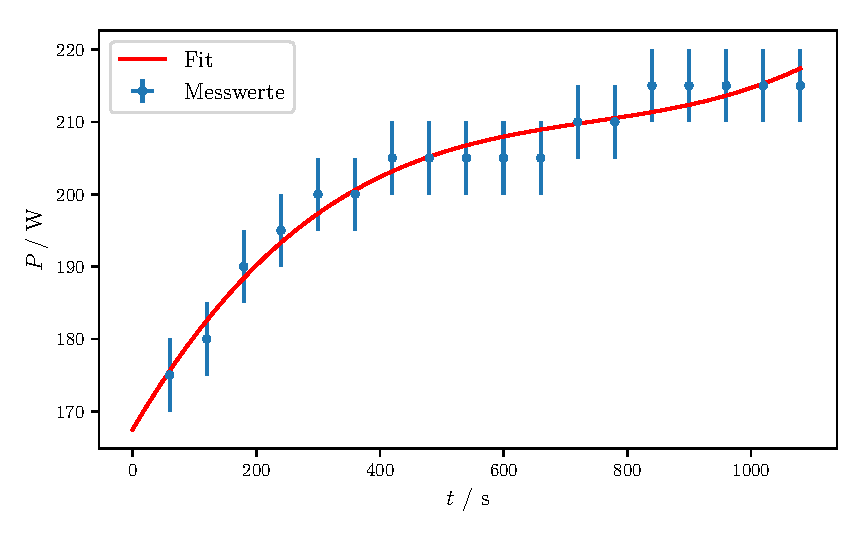
\includegraphics{plot-t-P.pdf}
  \caption{Die elektrische Leistung am Kompressor zu den jeweiligen Zeitpunkten.}
  \label{fig:plot_zeit-druck}
\end{figure}